% !TeX root = ../main.tex

\chapter{系统概要设计}

根据在上一章中介绍的系统需求,本章将对系统进行概要设计。首先对系统架
构进行设计,然后对系统的功能模块进行划分和设计,通过实体关系图详细介绍各个模块的数据库设计。

\section{系统总体设计}

本系统的目标在于构建一套一站式的数据入湖及数据分析探索的产品,提供数据入湖、
数据源管理、元数据管理、数据探索等方面的功能,并在元数据管理中添加了数据优化
的功能,解决了小文件合并等问题,目的是为用户降低学习成本和维护成本,提高数据使用人员的开发效率。

本系统采取计算与存储分离架构,使用的底层数据湖引擎为Apache Iceberg,
Iceberg具有事务语义、快照读写分离、数据修复、时间旅行等优势特性,提供
一站式数据入湖服务。湖上元数据可统一管理,无缝对接Spark、Presto、Flink
等引擎,可轻松完成T+0实时入湖,支持批流融合分析,挖掘和探索数据价值。旨在
构建新一代全场景实时数仓-数据湖分析系统,形成新一代大数据解决方案。

\subsection{功能架构设计}

功能架构包括数据湖底层引擎、数据湖管理及分析、数据湖交互分析及应用三层架构:

(1)数据湖底层引擎以iceberg为核心,提供表格式引擎。对下,支持HDFS、Ozone、COS内部使用最多三种存储引擎,
对上同Spark、Flink、Presto等实现无缝对接,通过Alluxio实现数据湖加速;

(2)基于数据湖底层核心,搭建数据湖管理与分析层,主要实现入湖管理、湖仓管理、数据湖计算分析关键及异常管理三大核心功能;

(3)支持强大的数据湖交互式分析及应用,同现有SuperSQl、Idex产品无缝对接,实现一站式湖仓数据查询及分析。
同时与传统BI产品、传统数据及APP应用对接,支持更多交互式分析场景。

数据湖分析平台支持各类异构数据源,包括传统关系型数据库(Mysql等)、流式数据及日志数据(Kafka、TubeMQ、Pulsar等)、
传统文件类型的数据源,基于流式计算平台Oceanus实现实时数据入湖任务,通过US实现存量数据入湖任务,实现一站式入
湖任务管理及分析。功能架构图如图4.1所示:

\begin{figure}[h]
  \centering
  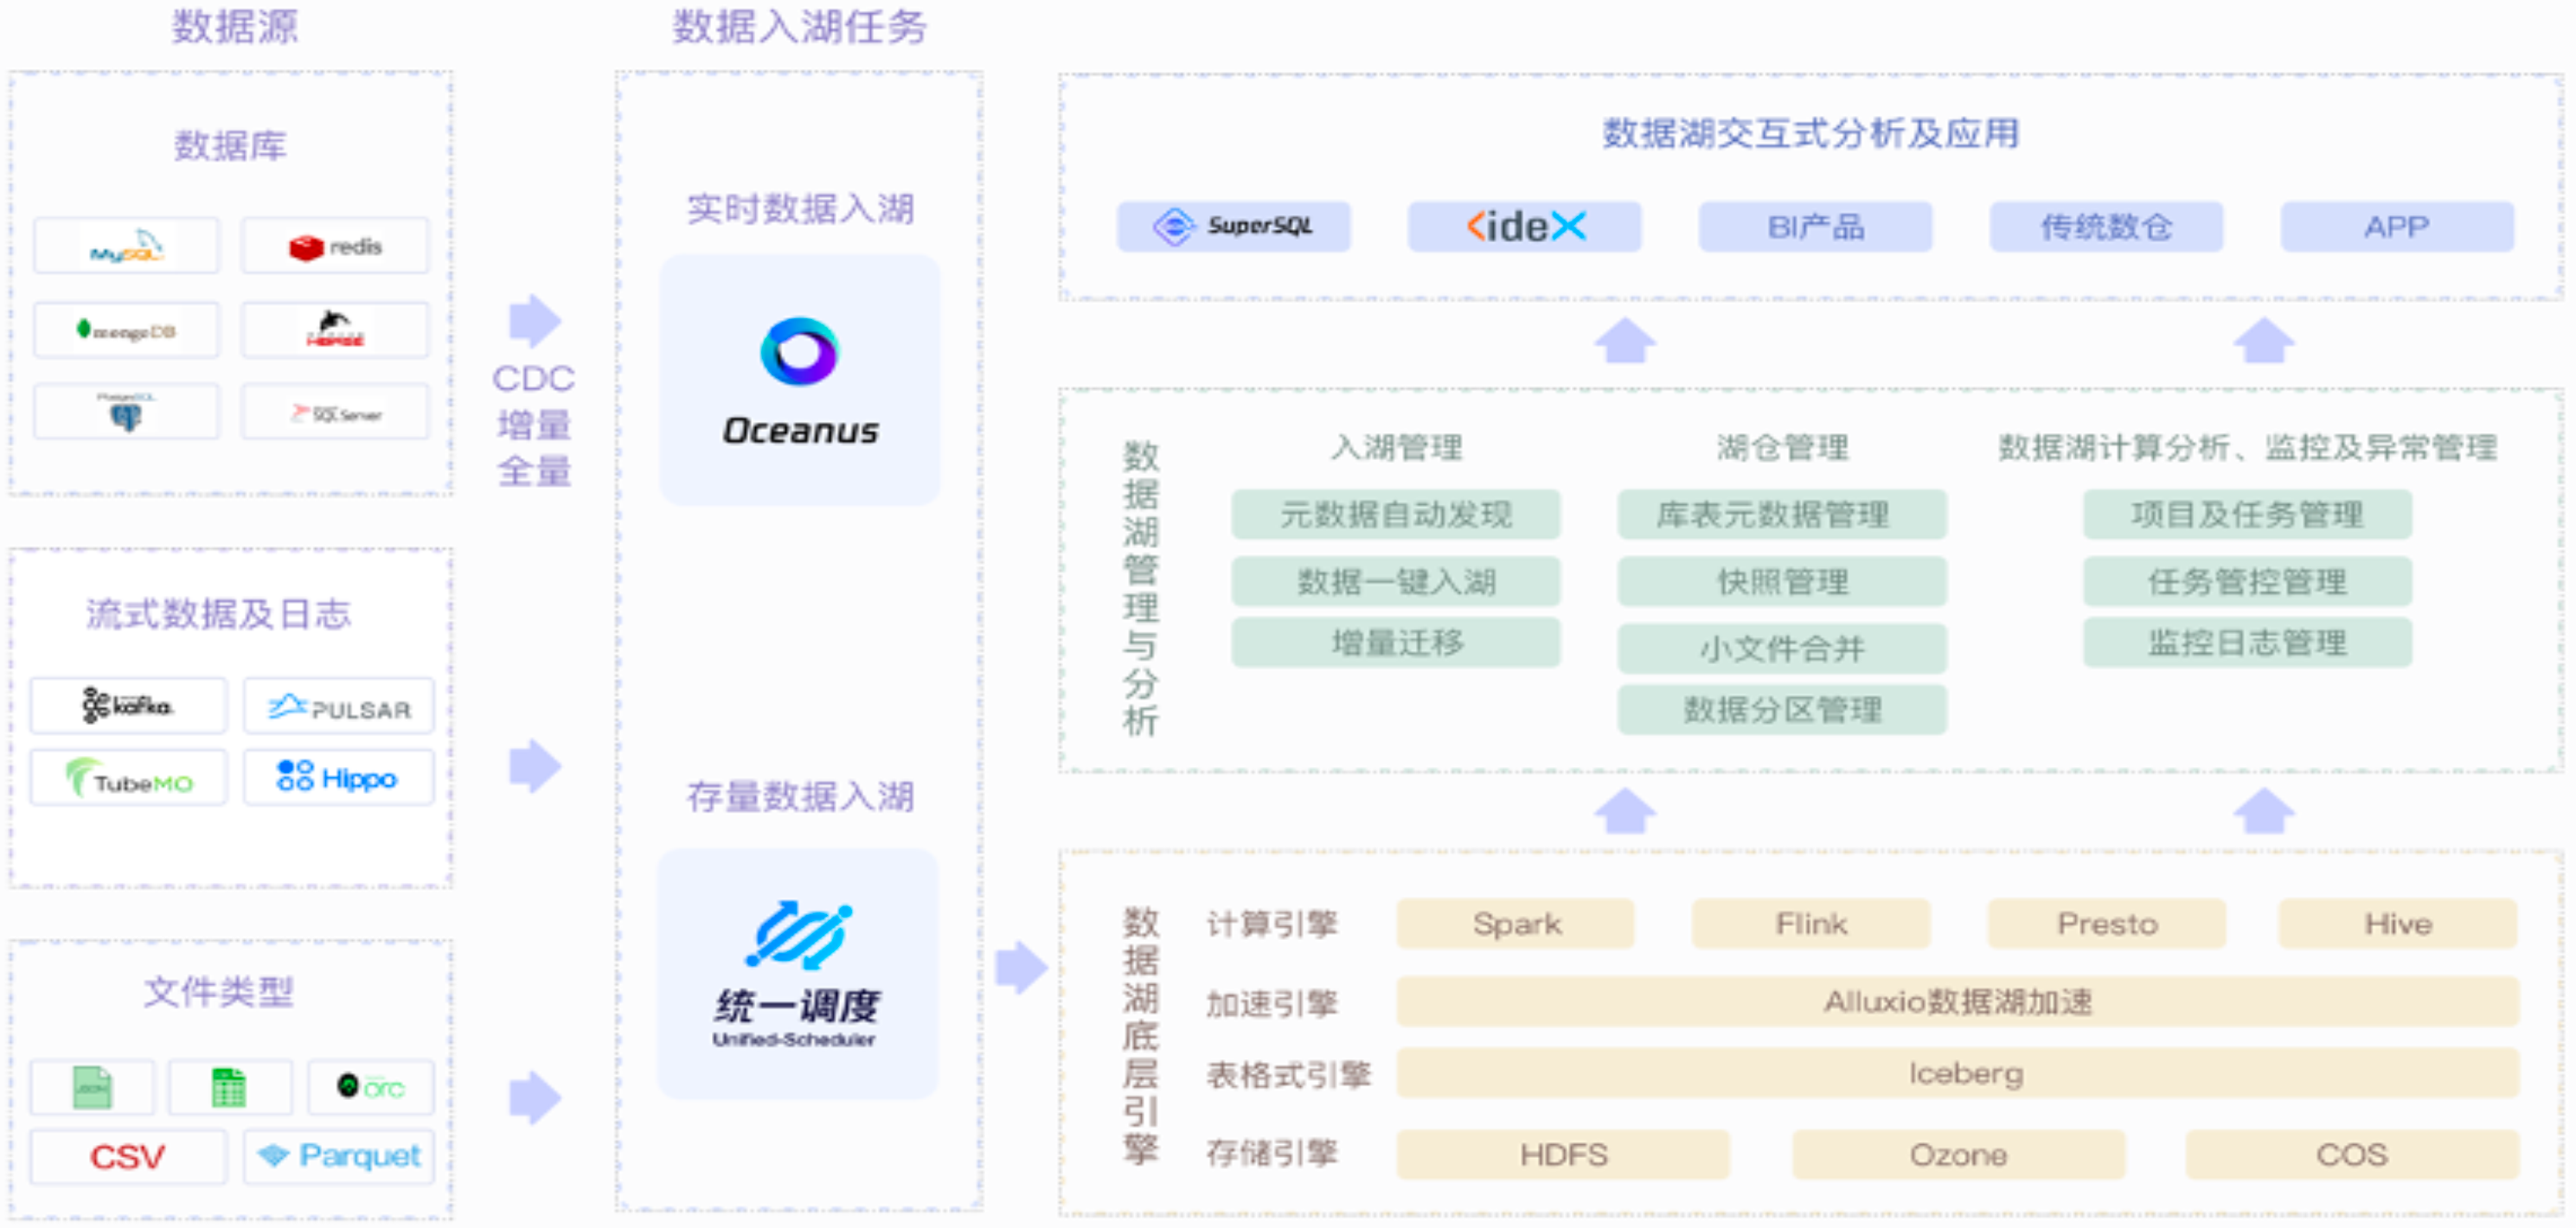
\includegraphics[width=1.0\textwidth]{功能架构图.png}
  \caption{功能架构图}
  \label{fig:badge}
\end{figure}

\subsection{系统架构设计}

数据湖分析系统的主要系统架构如图4.2所示。用户通过浏览器的前端页面访问服务器,服务器根据收到的请求进行业务层操作,
并对数据库持久层进行更新。该系统共有数据源管理、元数据管理管理、数据入湖管理、数据探索四个模块。
系统的数据持久能力主要由Mysql作为系统的数据库提供。

\begin{figure}[h]
  \centering
  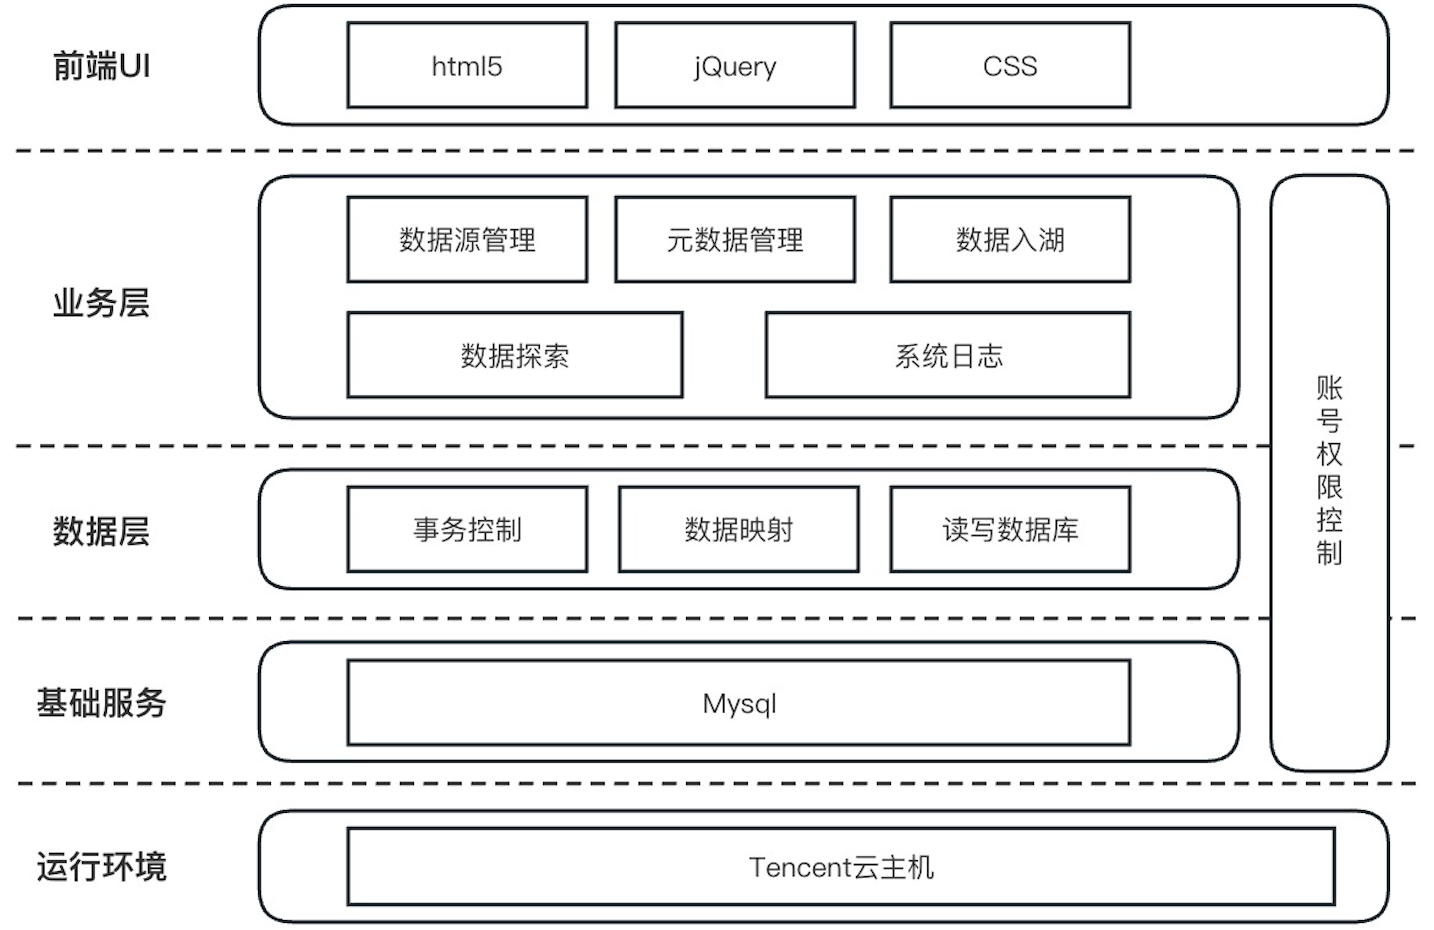
\includegraphics[width=1.0\textwidth]{系统架构图.png}
  \caption{系统架构图}
  \label{fig:badge}
\end{figure}

\section{系统功能模块设计}

根据上一章对数据湖分析系统的需求分析,将系统划分了四个模块:数据源管理、元数据管理、数据入湖、数据探索,
本节我们将对这四个功能模块和小文件合并优化功能进行设计。

\subsection{数据源管理模块}

数据源是入湖任务必须设置的,是Iceberg入湖的源头,从数据源分类上来看,
数据湖分析系统支持关系型数据库源(mysql)以及消息队列数据源(tube、kafka、pulsar),
该模块支持数据源创建、查看、编辑、删除功能,各数据源需要的信息字段如下:

(1)创建mysql数据源需要的信息字段如表4.1所示:

\begin{table}[h]
  \centering
  \caption{mysql数据源需要的信息字段}
  \label{tab:exampletable}
  \begin{tabular}{clcl}
    \toprule
    序号  & 字段名     & 是否空值   & 说明    \\
    \midrule
    1    & 数据源名称  & N        & 入湖任务通过mysql数据源名称(表名)指向mysql中的表 \\
    2    & 描述       & Y        & 对数据源的描述                                \\
    3    & 用户名     & N        & 与mysql用户名一致                             \\
    4    & 密码       & N        &  与mysql密码一致                             \\
    5    & 库名       & N        &   mysql中要入湖的数据库                       \\
    6    & 服务器地址  & N        &  可以是ip或者能解析的域名                      \\
    7    & 服务器端口  & N        &   mysql数据库端口号                          \\
    \bottomrule
  \end{tabular}
\end{table}

(2)创建tube数据源需要的信息字段如表4.2所示:

\begin{table}[h]
  \centering
  \caption{tube数据源需要的信息字段}
  \label{tab:exampletable}
  \begin{tabular}{clcl}
    \toprule
    序号  & 字段名     & 是否空值   & 说明                                      \\
    \midrule
    1    & 数据源名称  & N        & 入湖任务通过TUBE数据源名称指向tube中的表 \\
    2    & 描述       & Y        & 对数据源的描述                                \\
    3    & TUBE业务ID     & N        & TUBE业务ID名称                             \\
    4    & TUBE服务器列表       & N        &  系统填充,输入正确的TUBE业务ID后会自动填充对应的列表         \\
    \bottomrule
  \end{tabular}
\end{table}

(3)创建kafka数据源需要的信息字段如表4.3所示:

\begin{table}[h]
  \centering
  \caption{kafka数据源需要的信息字段}
  \label{tab:exampletable}
  \begin{tabular}{clcl}
    \toprule
    序号  & 字段名     & 是否空值   & 说明                                      \\
    \midrule
    1    & 数据源名称  & N        & 入湖任务通过kafka服务器地址指向kafka中的表 \\
    2    & 描述       & Y        & 对数据源的描述                               \\
    3    & Kafka服务地址    & N        & kafka服务地址                           \\
    4    & Kafka版本号      & N        &  kafka版本号       \\
    \bottomrule
  \end{tabular}
\end{table}

(4)创建Pulsar数据源需要的信息字段如表4.4所示:

\begin{table}[h]
  \centering
  \caption{Pulsar数据源需要的信息字段}
  \label{tab:exampletable}
  \begin{tabular}{clcl}
    \toprule
    序号  & 字段名     & 是否空值   & 说明                                      \\
    \midrule
    1    & 数据源名称  & N        & 入湖任务通过Pulsar服务器地址指向Pulsar中的表 \\
    2    & 描述       & Y        & 对数据源的描述                               \\
    3    & Pulsar业务ID    & N        & Pulsar业务ID                          \\
    4    & Pulsar服务地址      & N        &  系统填充,输入正确的Pulsar业务ID后会自动填充对应的服务地址      \\
    \bottomrule
  \end{tabular}
\end{table}

\subsection{元数据管理模块}

元数据模块是用来管理iceberg表元数据的,包含四个主要的功能,分别是表的创建、表的编辑、表的查看、数据优化。

其中表的创建需要和hive metastore、mysql进行交互,一个createTable的request建立后,
首先会判断metastore中是否已存在表,若不存在,则会判断MySQL中是否存在对应的DB和table,
这里MySQL中的DB和table实质上是一个映射,是用来方便在DLA展示表元数据的,若MySQL中不存在,
则创建对应的DB和table,接着会在metastore中创建实际的iceberg表元数据;表的查看直接去
MySQL中查看即可;表的编辑如果涉及到字段的增加及删除操作,则会更新metastore中对应的
表元数据。创建Iceberg表的时序图如图4.3所示。

\begin{figure}[h]
  \centering
  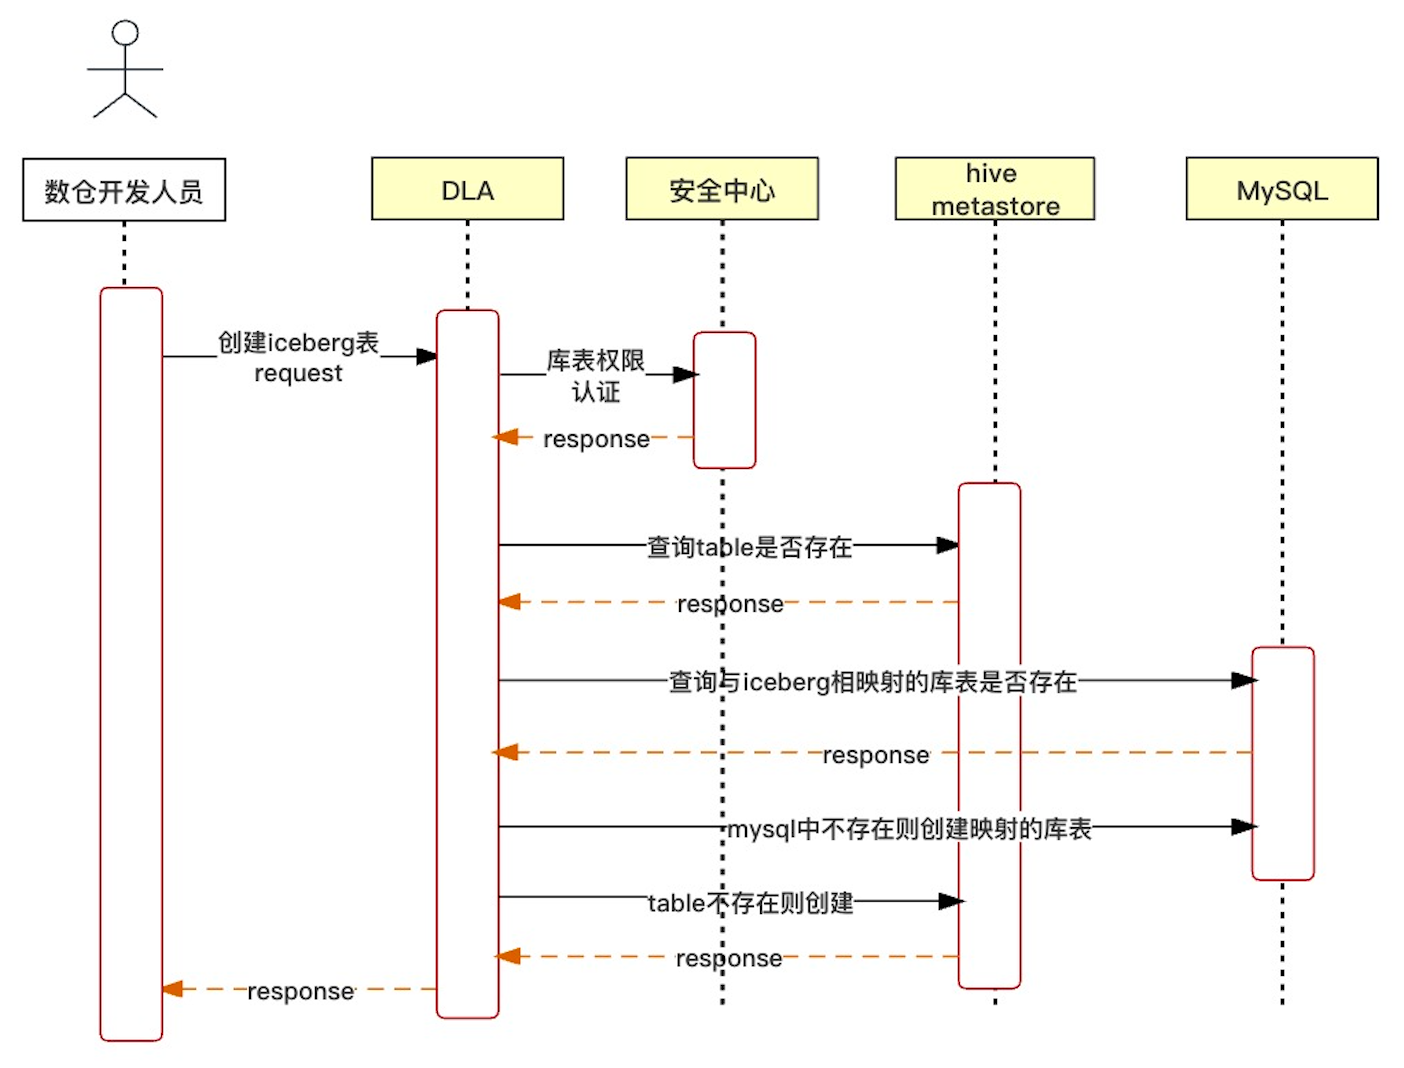
\includegraphics[width=1.0\textwidth]{DLA创建Iceberg表时序图.png}
  \caption{DLA创建Iceberg表时序图}
  \label{fig:badge}
\end{figure}

数据优化是一个服务,目的是减少用户的iceberg运维成本和学习成本,它能够帮助用户一键式优化。
当前的功能包括小文件合并、历史元数据清理、孤儿文件删除、数据生命周期管理,其中我们在小文件
合并这方面做了很多的优化,会在接下来的章节进行介绍。在DLA中,用户可以一键启动优化服务,并
可配置开启某些功能,以及一些文件大小和过期时间配置。其功能结构图如图4.4所示。

\begin{figure}[h]
  \centering
  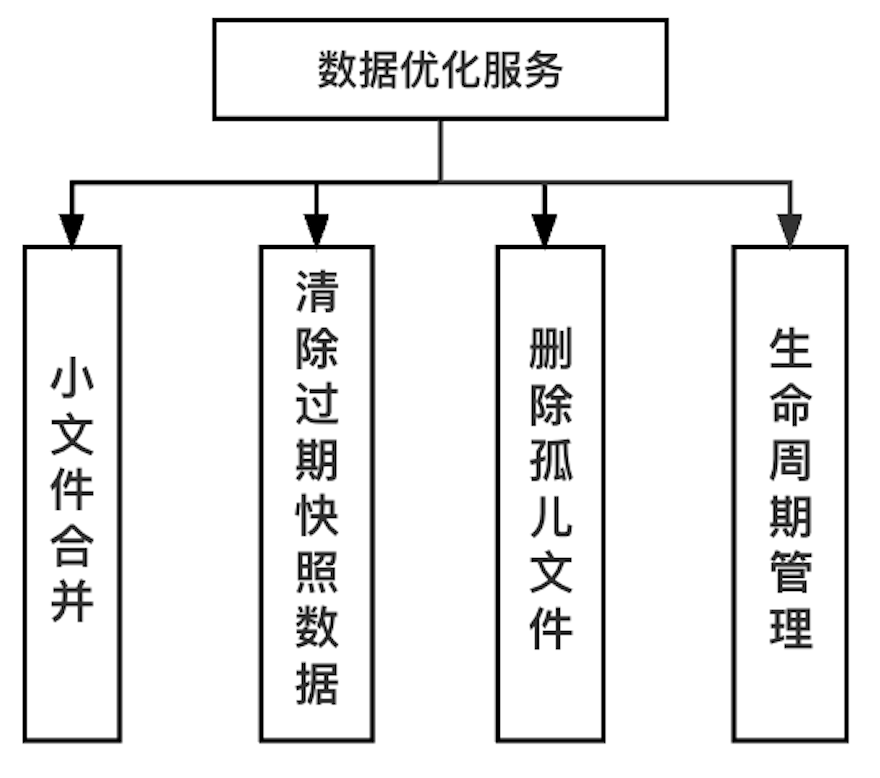
\includegraphics[width=1.0\textwidth]{数据优化服务功能结构图.png}
  \caption{数据优化服务功能结构图}
  \label{fig:badge}
\end{figure}

\subsection{数据入湖模块}

数据入湖功能模块是DLA系统核心流程功能,目的是用户通过该功能将源数据表流程化入湖
和查看已申请入湖任务执行情况。入湖任务分为三类,分别为实时数据入湖、存量数据入湖
和关系型数据入湖,三类入湖任务的创建都需要填写基础信息、源表、目标表、参数及资源,
若目标表在任务创建的时候还没有创建,则会自动的根据填写的字段信息生产对应的目标表,
即在对应的数据库中生成iceberg表。该模块的时序图如图4.5所示。

入湖任务都会生成对应的jar包,若为实时数据入湖,则会在公司内部的实时流计算平台
Oceanus上创建对应的jar任务,底层使用的引擎是flink;若为存量数据入湖或者关系
型数据入湖,则会在定时任务执行平台US上创建jar任务,底层使用的引擎是spark,
并可在DLA上设置任务执行的时间间隔和起始时间。

\begin{figure}[h]
  \centering
  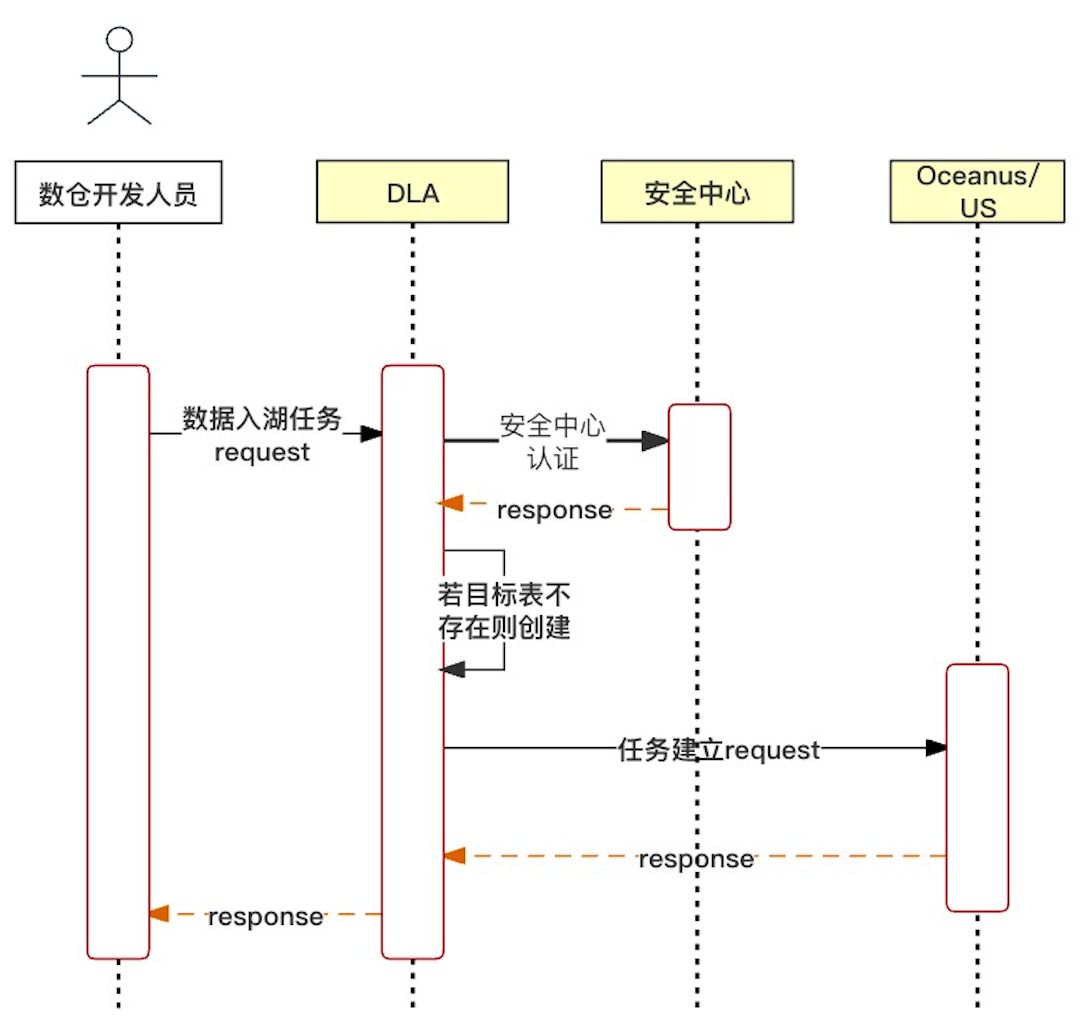
\includegraphics[width=1.0\textwidth]{入湖任务创建时序图.png}
  \caption{入湖任务创建时序图}
  \label{fig:badge}
\end{figure}

\subsection{数据探索模块}

数据探索功能是数据入湖后,用户需要进行数据查看或者数据分析时使用的工具,
目前主要依赖内部平台IDEX实现数据探索功能,在该平台上,用户可以编写sql
设置执行引擎,presto或者spark。其中presto查询速度快,但是功能少,
只支持查询功能;spark虽然查询速度慢,但支持的语句功能比较多,支持创建表、
删除表、更新表、数据写入、数据删除、更新分区、表维护等语句。在IDEX上的数据探索时序图如图4.6所示。

除了IDEX平台可以进行数据探索外,我们还提供了Zeppelin可以进行数据探索,
Zeppelin是一个基于Web的notebook,提供交互数据分析和可视化。后台支持接
入多种数据处理引擎,如spark,hive等。支持多种语言: Scala(Apache Spark)、
Python(Apache Spark)、SparkSQL、 Hive、 Markdown、Shell等。开发者可以通过实现更多的解释器来为Zeppelin添加数据引擎。

\begin{figure}[h]
  \centering
  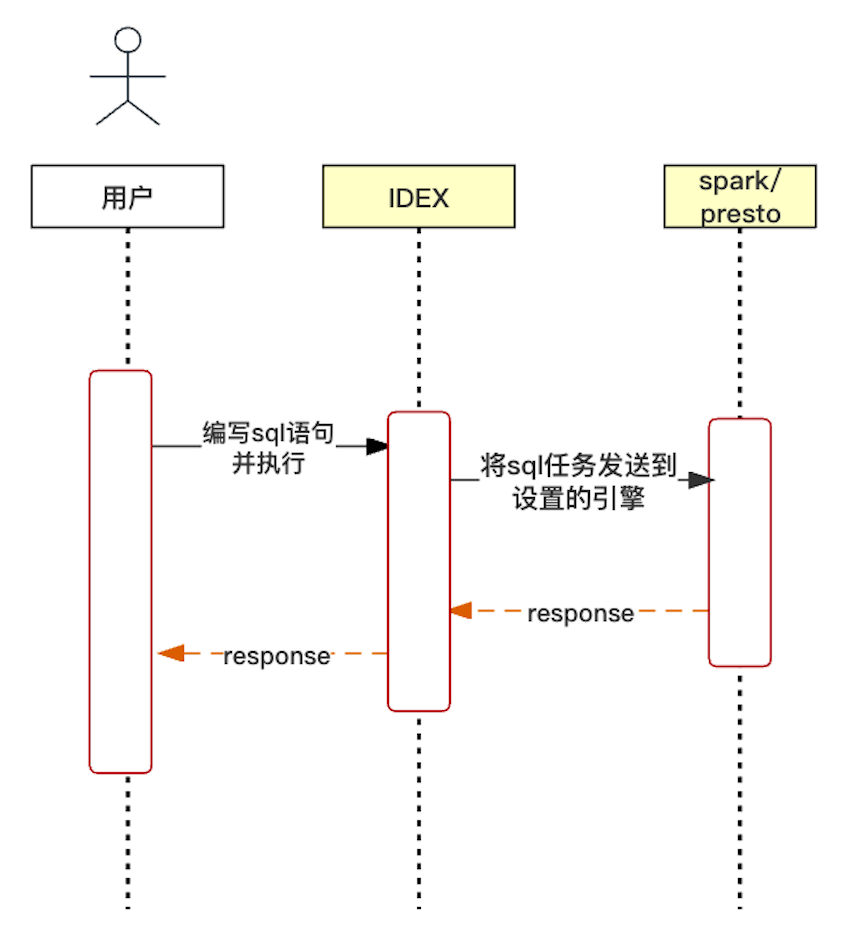
\includegraphics[width=1.0\textwidth]{数据探索时序图.png}
  \caption{数据探索时序图}
  \label{fig:badge}
\end{figure}

\subsection{小文件合并优化模块}

我们重新设计了小文件合并模块,因为原有的Iceberg小文件合并功能在实际应用中存在很多问题,如合并不及时、浪费资源以及占用计算资源过多等。

\subsubsection{分区表进行重分区}

对于重分区的功能实现,只需要在inputStream后进行一个KeyBy Partition操作就能解决,
这个操作相当于是根据Partition对数据进行了一个分组,然后在将这些分好组的数据分别交给对应的
IcebergWriter来进行写入,如图4.7所示。

\begin{figure}[h]
  \centering
  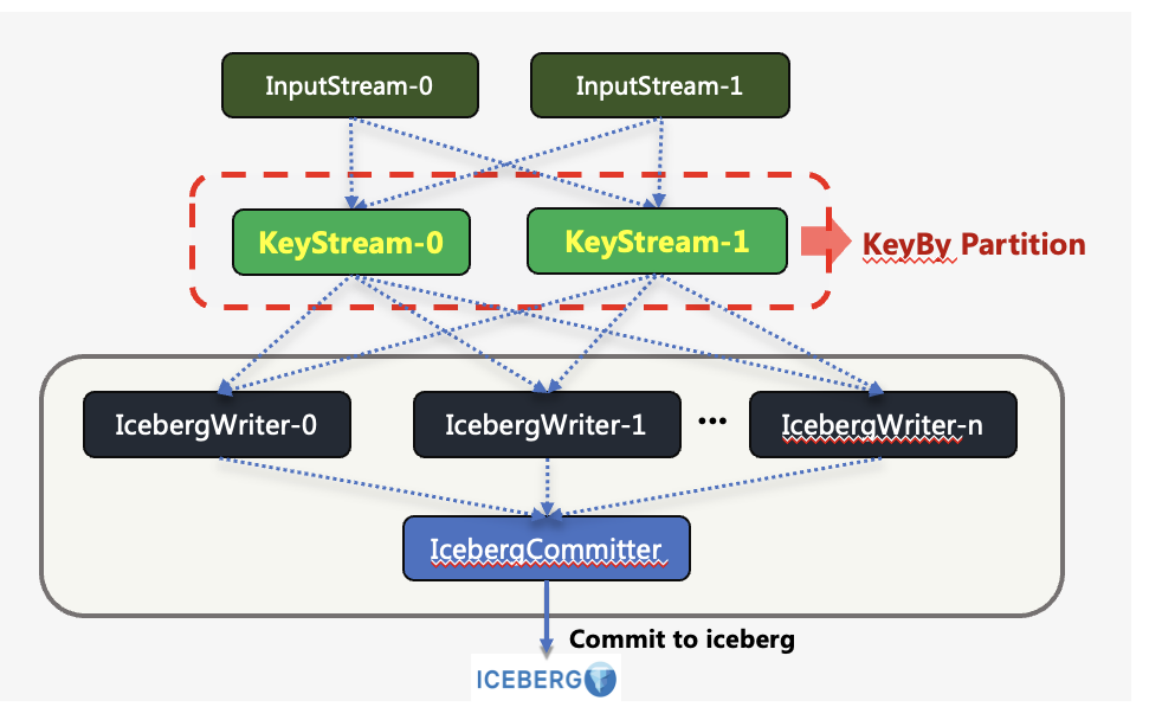
\includegraphics[width=1.0\textwidth]{进行重分区的Iceberg写入示意图.png}
  \caption{进行重分区的Iceberg写入示意图}
  \label{fig:badge}
\end{figure}

经过这样的优化之后,我们可以看到图4.8和4.9效果,磁盘上的文件分布即每个writer
只会写其负责的那部分分区数据,且writer 之间不会存在分区数据重叠,这样分区前后
的文件数量大大减少。当前提供了一个参数“write-distribute-mode”进行配置,
如果用户表是一个分区表,则可以在Flink任务代码中将这个参数设置成hash
(当前只支持hash分区模式),该参数为 Flink 作业的参数。

\begin{figure}[h]
  \centering
  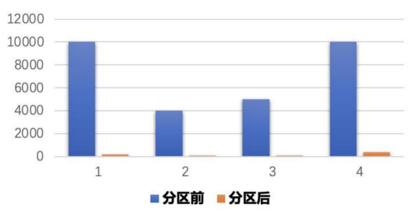
\includegraphics[width=1.0\textwidth]{重分区前后小文件数量对比.png}
  \caption{重分区前后小文件数量对比}
  \label{fig:badge}
\end{figure}

\begin{figure}[h]
  \centering
  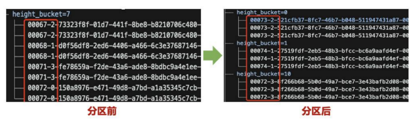
\includegraphics[width=1.0\textwidth]{重分区前后分区文件分布.png}
  \caption{重分区前后分区文件分布}
  \label{fig:badge}
\end{figure}

\subsubsection{小文件合并优化}

由于合并的任务无法知道当前的文件状态,因此需要一种计算规则来判断当前一个区间内
是否达到了发起合并任务的时刻,即需要计算出文件的状态,以作为合并任务调度的合并规则。这里我们采用的是均方误差的计算方法。

均方误差(MSE)的数学含义是表示一个样本区间内样本值与目标值之间差异程度的一种度量,
我们设定合并后大文件的目标大小为512MB,则这个样本区间就是512MB,如果MSE的值越大,
表示当前样本区间内的文件相对于目标大小的差值也越大,因此我们可以设定一个阈值来决定合并的粒度,
例如设置一个T,当T 越大表示合并的区间内小文件的比例要越高才会被触发到合并。如图4.10所示。
MSE通过公式4.1进行计算:

\begin{equation}
  MSE=\frac {\sum_{i=1}^{N}{(Target_i - Actual_i)^2}} {N}
  \label{eq:example}
\end{equation}

其中N代表一个分区内的文件数,Target代表合并后的目标文件大小,Actual 等于min(分区内实际的文件大小, Target)。

当分区内文件状态需要更新的时候,通过公式4.2和公式4.3进行计算:

\begin{equation}
  SE=\sum_{i=1}^{N}{(Target_i - Actual_i)^2}
  \label{eq:example}
\end{equation}

其中M代表分区内的新的文件数。

\begin{equation}
  MSEnew=\frac {MSEold*N+SE} {N+M}
  \label{eq:example}
\end{equation}

阈值T的取值通过公式4.4进行计算:

\begin{equation}
  T=(Target*a)^2 \qquad (0<a<1)
  \label{eq:example}
\end{equation}

\begin{figure}[h]
  \centering
  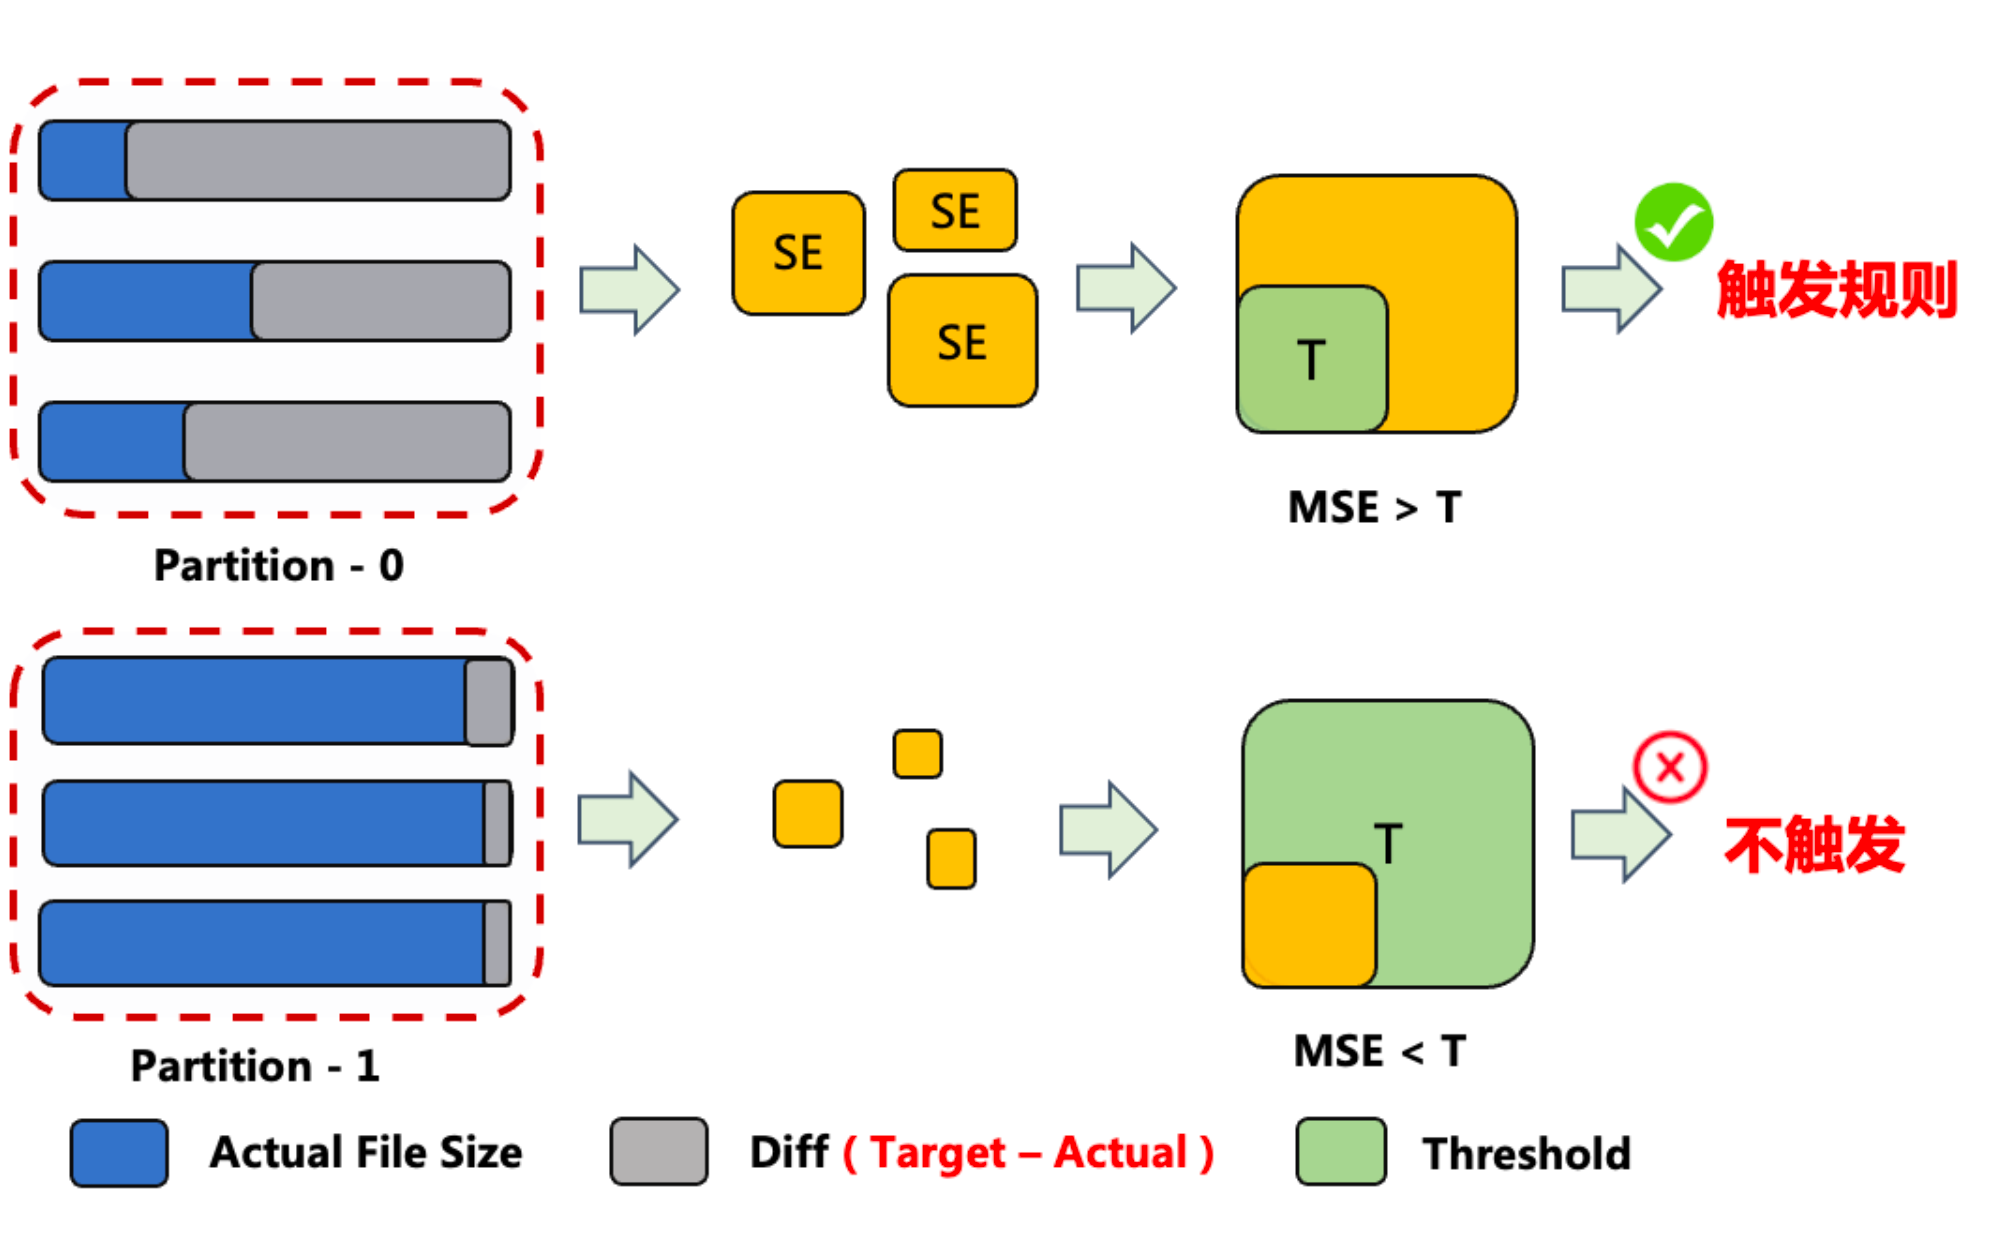
\includegraphics[width=1.0\textwidth]{小文件合并触发示意图.png}
  \caption{小文件合并触发示意图}
  \label{fig:badge}
\end{figure}

计算后得到的MSE的值之后,通过事件汇报的方式发送到文件合并服务,后台服务在收到这些
MSE之后自动根据不同的表所配置的不同的值来决策是否需要对某个分区或者是某张表进行合并。
commit 事件为一次snapshot 生成的事件,通过计算每个snapshot里面的文件状态并通过
summary 的方式记录通过事件发送到后端服务,从而使得服务能够清楚的了解当前每一张表的
snapshot中的文件状态,以此来作为是否触发合并的判断依据,Iceberg Commit事件结构如图4.11所示。

\begin{figure}[h]
  \centering
  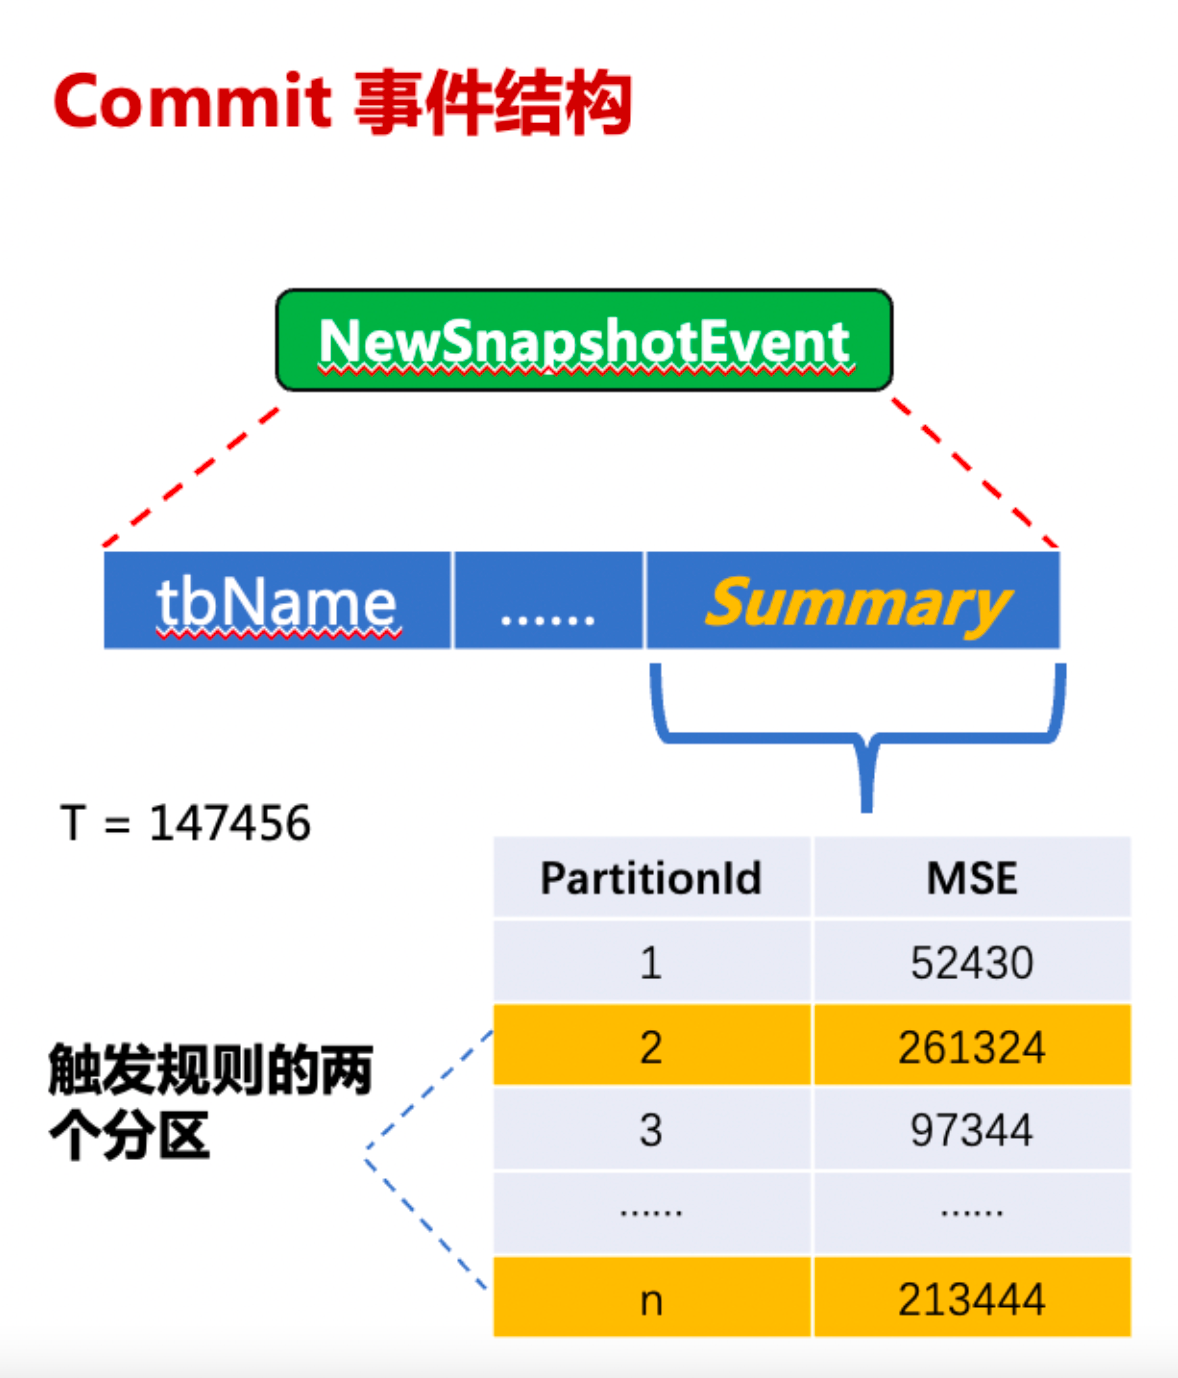
\includegraphics[width=1.0\textwidth]{Iceberg Commit事件结构.png}
  \caption{Iceberg Commit事件结构}
  \label{fig:badge}
\end{figure}

经过这样的优化后,如图4.12所示,合并优化的文件状态均在一个均衡的水平,
小文件的增长得到了有效的控制,离线合并任务只在MSE达到某个阈值的时候才触发合并,避免了不必要的计算资源的开销。

\begin{figure}[h]
  \centering
  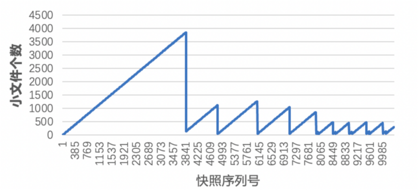
\includegraphics[width=1.0\textwidth]{随着时间的执行小文件个数的变化.png}
  \caption{随着时间的执行小文件个数的变化}
  \label{fig:badge}
\end{figure}

\section{系统数据库设计}

在信息存储方面,DLA主要使用mysql进行信息存储,主要包括任务信息、任务详情信息、
目标库信息、目标表信息、数据源信息、任务jar包信息,其中目标库和目标表在mysql
中的信息只是一个映射,具体实际的表还是Iceberg表,其数据存储在HDFS集群上。数据库ER图如图4.13所示。

\begin{figure}[h]
  \centering
  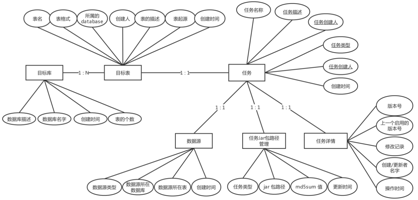
\includegraphics[width=1.0\textwidth]{数据库ER图.png}
  \caption{数据库ER图}
  \label{fig:badge}
\end{figure}

系统中主要的数据库表格结构设计如下:

(1)任务表(dlaTask)详细描述如表4.5所示。

\begin{table}[h]
  \centering
  \caption{任务表}
  \label{tab:exampletable}
  \begin{tabular}{clllcl}
    \toprule
    序号  & 字段名         & 字段说明     & 类型           & 是否可为空   & 说明  \\
    \midrule
    1    & id            & 任务id      & bigint(20)     & N          & PRIMARY KEY    \\
    2    & name          & 任务名称     & varchar(256)   & N          &     \\
    3    & desc          & 任务描述     & text           & Y          &   \\
    4    & tableId       & 目标表id     & bigint(20)     & N          &   \\
    5    & type          & 任务类型     & tinyint(4)     & N          & 1-Oceanus实时  \\
         &               &             &               &             & 2-US存量  \\
    6    & actualTaskId  & 实际的任务id  & bigint(20)    & N          &  1-Oceanus任务id  \\
         &               &             &               &             & 2-US任务id  \\
    7    & creatorName   & 创建者       & varchar(64)    & N          &   \\
    8    & createTime    & 创建时间     & timestamp      & N          &   \\
    9    & deleted       & 是否被删除    & boolean        & N          &   \\
    10   & numRetries    & 重试次数      & int(4)        & N          &   \\
    \bottomrule
  \end{tabular}
\end{table}

(2)任务详情表(dlaTaskDetail)详细描述如表4.6所示。

\begin{table}[h]
  \centering
  \caption{任务详情表}
  \label{tab:exampletable}
  \begin{tabular}{clllcl}
    \toprule
    序号  & 字段名              & 字段说明     & 类型           & 是否可为空   & 说明  \\
    \midrule
    1    & id                 & 任务详情id   & bigint(20)     & N          & PRIMARY KEY    \\
    2    & taskId             & 任务id      & bigint(20)     & N          &    \\
    3    & version            & 任务版本     & bigint(10)     & N          &   \\
    4    & lastEffectVersion  & 上一个版本   & bigint(10)     & N          &   \\
    5    & modification       & 修改记录     & text           & Y          &   \\
    6    & updateUser         & 更新者       & varchar(64)   & N          &    \\
    7    & updateTime         & 操作时间     & timestamp      & N          &   \\
    8    & taskDetail         & 任务详情     & text           & N          &   \\
    9    & complete           & 是否提交     & boolean        & N          &   \\
    \bottomrule
  \end{tabular}
\end{table}

(3)目标库(dlaDatabase)详细描述如表4.7所示。

\begin{table}[h]
  \centering
  \caption{目标库}
  \label{tab:exampletable}
  \begin{tabular}{clllcl}
    \toprule
    序号  & 字段名              & 字段说明     & 类型           & 是否可为空   & 说明  \\
    \midrule
    1    & id                 & 目标库id     & bigint(20)    & N          & PRIMARY KEY    \\
    2    & name               & 数据库名称    & varchar(256)  & N          &    \\
    3    & desc               & 数据库描述    & text          & Y          &   \\
    4    & tableNum           & 表的个数      & Int           & N          &   \\
    5    & createTime         & 创建时间      & timestamp     & N          &   \\
    \bottomrule
  \end{tabular}
\end{table}

(4)目标表(dlaTable)详细描述如表4.8所示。

\begin{table}[h]
  \centering
  \caption{目标表}
  \label{tab:exampletable}
  \begin{tabular}{clllcl}
    \toprule
    序号  & 字段名              & 字段说明     & 类型           & 是否可为空   & 说明  \\
    \midrule
    1    & id                 & 目标表id     & bigint(20)    & N          & PRIMARY KEY    \\
    2    & name               & 表名         & varchar(256)  & N          &    \\
    3    & format             & 表格式       & tinyint(4)    & N          & 1-iceberg  \\
         &                    &             &               &            & 2-hudi  \\
    4    & dbName             & 所属DB       & varchar(256)  & N          &   \\
    5    & creatorName        & 创建人       & varchar(64)   & N          &   \\
    6    & dataSourceId       & 数据源id     & bigint(20)    & Y          &    \\
    7    & desc               & 表的描述     & text           & Y          &   \\
    8    & origin             & 表起源       & tinyint(4)    & N          & 1-数据湖页面创建的表   \\
         &                    &             &               &            & 2-其他地方同步  \\
    9    & deleted            & 是否被删除    & boolean       & N          &   \\
    10   & createTime         & 创建时间     & timestamp     & N          &    \\
    11   & deleteTime         & 删除时间     & timestamp     & Y          &   \\
    \bottomrule
  \end{tabular}
\end{table}

(5)数据源表(dlaDatasource)详细描述如表4.9所示。

\begin{table}[h]
  \centering
  \caption{数据源表}
  \label{tab:exampletable}
  \begin{tabular}{clllcl}
    \toprule
    序号  & 字段名              & 字段说明           & 类型           & 是否可为空   & 说明  \\
    \midrule
    1    & id                 & 数据源id           & bigint(20)    & N          & PRIMARY KEY    \\
    2    & type               & 数据源类型          & smallint(8)   & N          & 1-Tube   \\
         &                    &                   &               &            & 2-Kafka  \\
         &                    &                   &               &            & 3-Pulsar  \\
         &                    &                   &               &            & 4-Mysql  \\
    3    & actualTableId      & 所对应的真实tableId  & bigint(20)   & N          &   \\
    4    & sourceDB           & 所在数据库          & varchar(256)  & N          &   \\
    5    & sourceTable        & 所在表             & varchar(256)  & N          &   \\
    6    & createTime         & 创建时间           & timestamp     & N          &    \\
    \bottomrule
  \end{tabular}
\end{table}

(6)任务jar包管理表(dlaTaskJar)详细描述如表4.10所示。

\begin{table}[h]
  \centering
  \caption{任务jar包管理表}
  \label{tab:exampletable}
  \begin{tabular}{clllcl}
    \toprule
    序号  & 字段名              & 字段说明           & 类型           & 是否可为空   & 说明  \\
    \midrule
    1    & id                 & 任务jar id        & bigint(20)     & N          & PRIMARY KEY    \\
    2    & type               & 任务类型           & tinyint(4)    & N           & 1-Oceanus实时   \\
         &                    &                   &               &            & 2-US存量   \\
    3    & jarPath            & jar包路径         & varchar(512)   & N          &   \\
    4    & md5sum             & md5sum校验值      & varchar(128)   & N          &   \\
    5    & updateTime         & 更新时间           & timestamp     & N          &   \\
    \bottomrule
  \end{tabular}
\end{table}

\section{本章小结}

本章主要阐述了数据湖分析系统的概要设计。首先介绍系统的总体架构,对
功能架构和系统架构进行了简单描述。另外根据上一章的需求分析,对系统的功能模块进行划分,并且详
细介绍了每个模块的功能设计。最后介绍了整个系统的数据库设计,展示数据库ER图以及主要的数据库表结构。

